%!TEX root = project_description.tex

%%%%%%%%%%%%%%%%%%%%%%%%%%%%%%%%%
\section{Timeline and Milestones}
\label{sec:timeline}
%%%%%%%%%%%%%%%%%%%%%%%%%%%%%%%%%

To be written...
% The timeline for this project is organized by three major tasks labeled Thrust \#1, Thrust \#2, and Thrust \#3, and also includes a timeline for broader impact activities.  Thrust \#1 investigates the syntax and semantics of a functional reactive programming language for chemical reaction networks.  Thrust \#2 investigates an LTL-based type system for the functional reactive programming language investigated in Thrust \#1.  Thrust \#3 iterates throughout the project to support software tools for Thrust \#1 and thrust \#2.  All of the thrusts, included the broader impact activities will be carried out simultaneously over the three years.  Theses thrusts are further divided into several tasks, and appear in the time line chart below.  A lead investigator(s) is also indicated for each task determined by the expertise of the investigator in the specific task.
% \begin{figure}[h!]
%     \centering
%     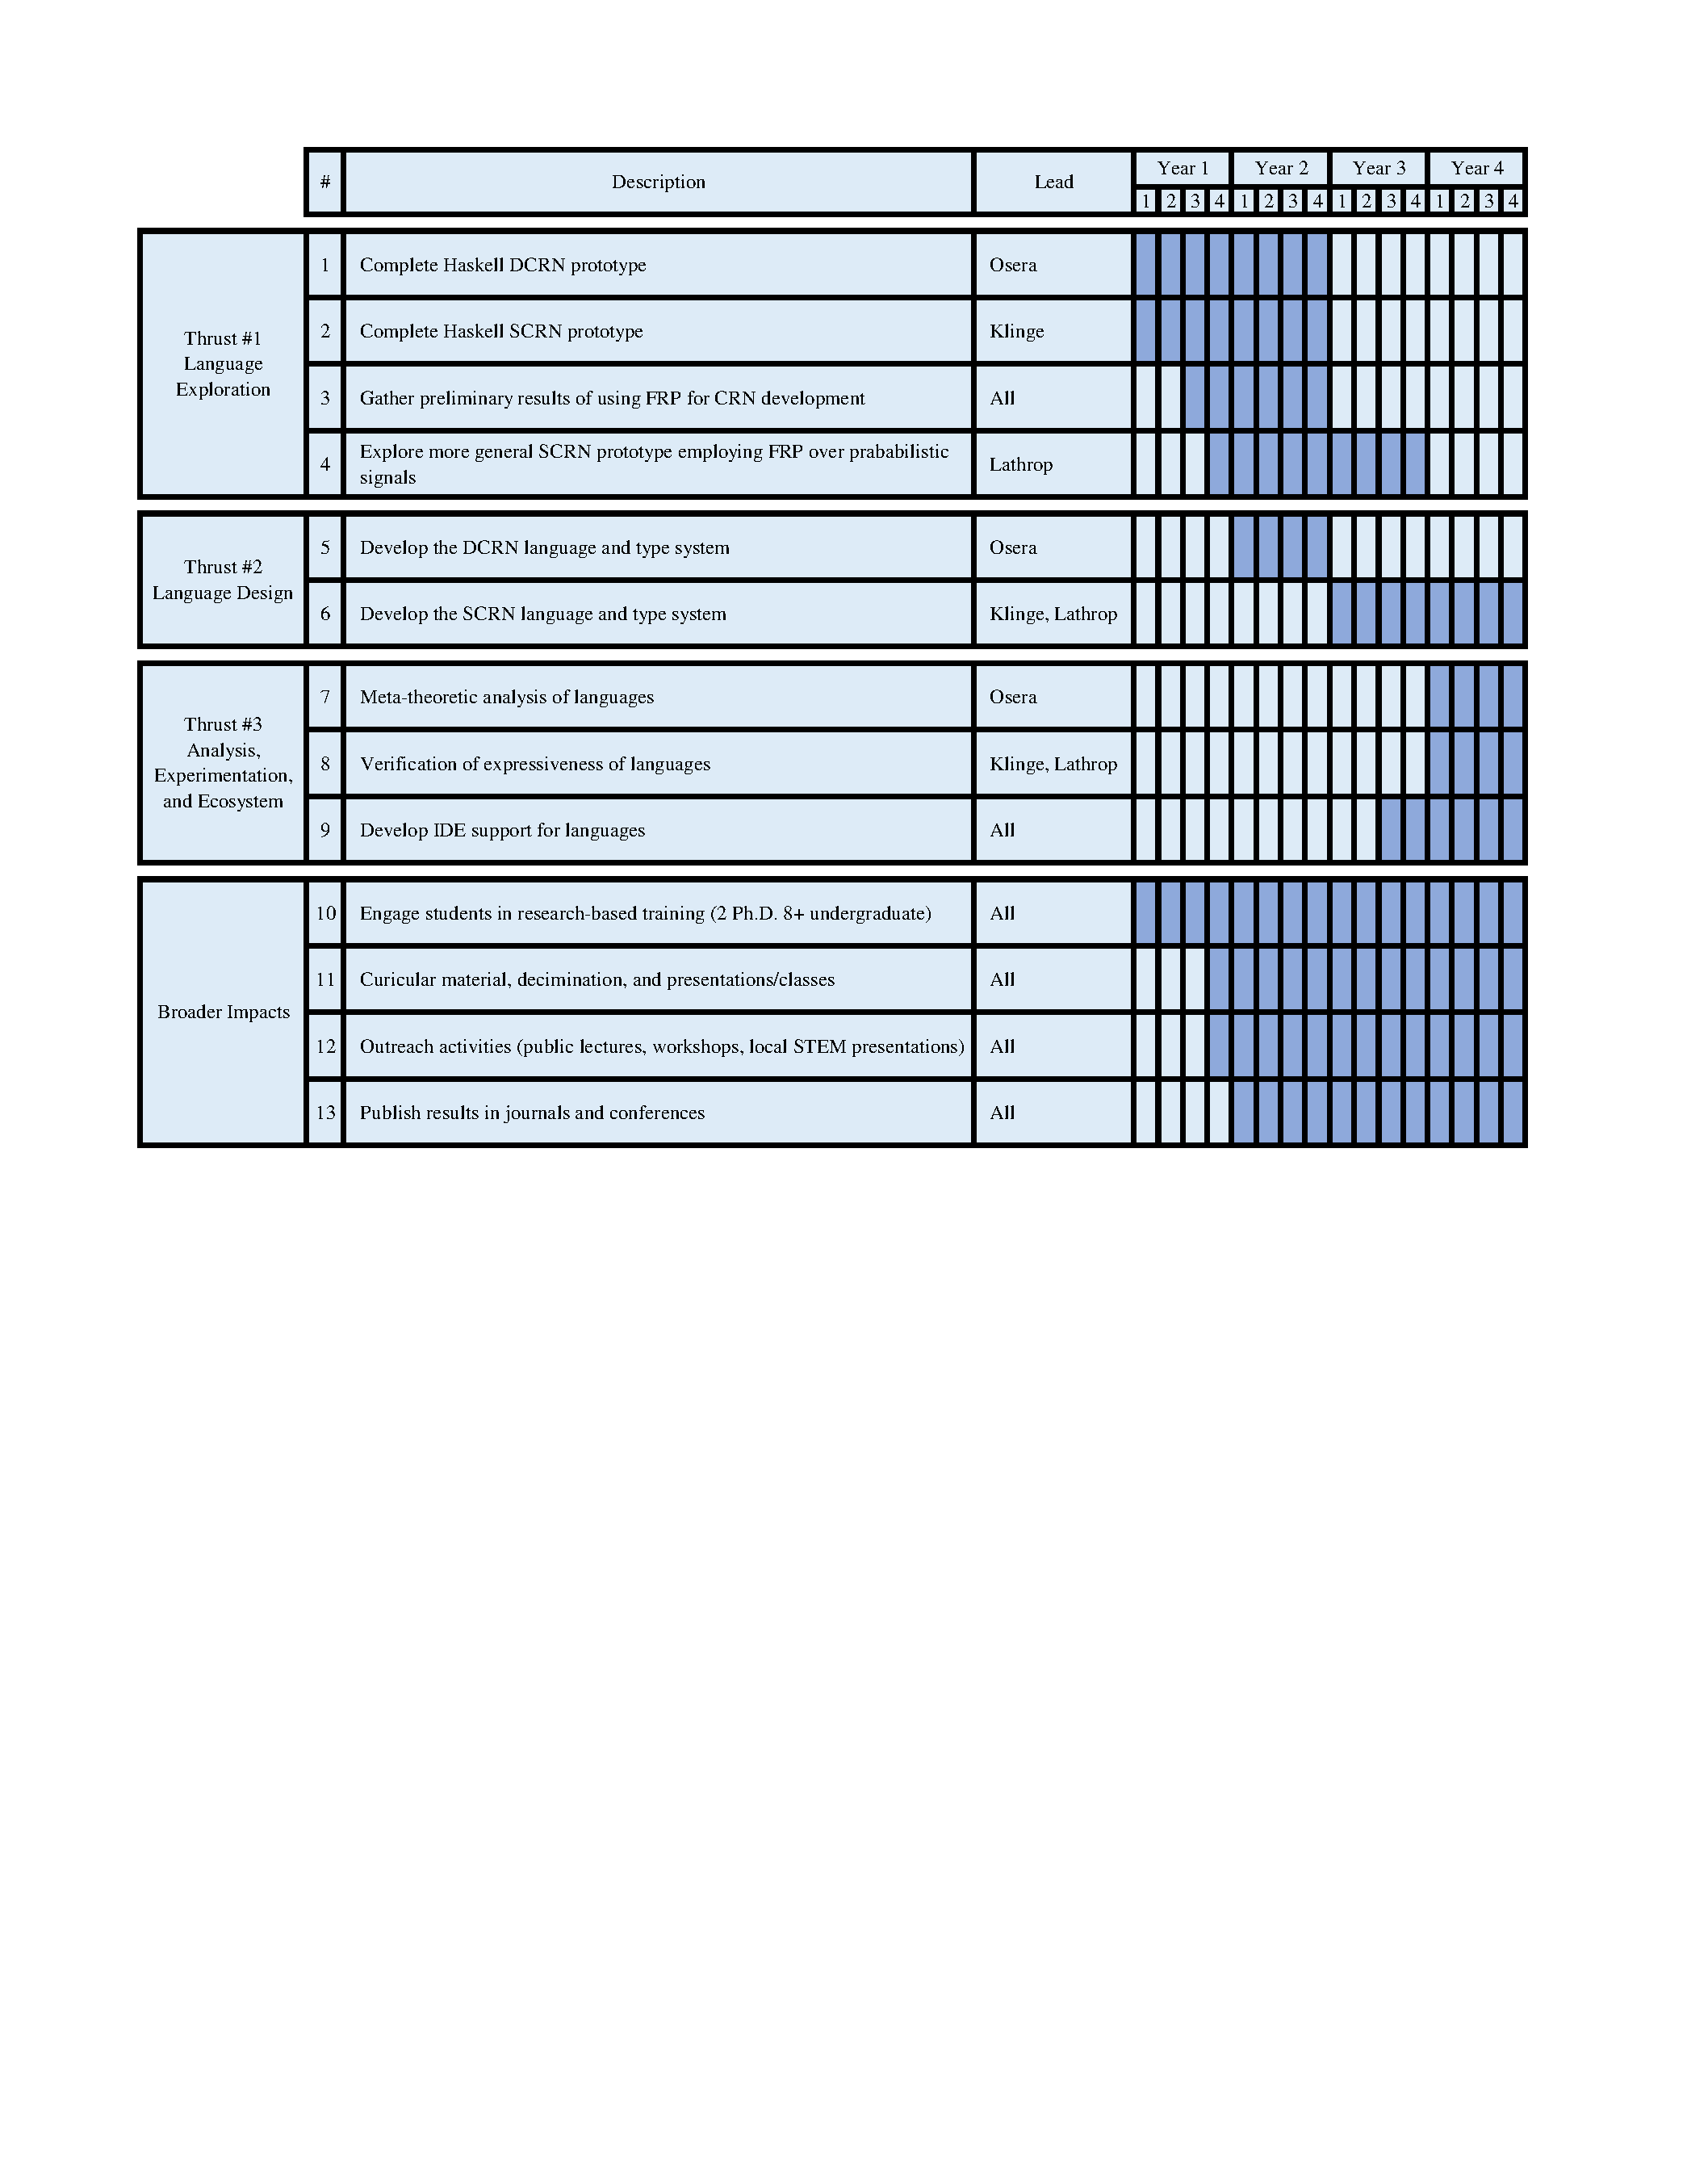
\includegraphics[width=6.4in]{TimeLine.pdf}
%     \caption{Timeline}
% \end{figure}


